\section{Experiment}
\label{sec:experiment}

\subsection{Datasets and Evaluation Metrics}
\label{subsec:datasets_metrics}

\subsubsection{Datasets}
\label{subsec:datasets}

We evaluate MgfrOFR on the SRWOV benchmark introduced with MambaOFR~\cite{mao2025mambaofr}. SRWOV is a dedicated old film restoration benchmark with both synthetic and real-world test sets.

Training uses the REDS training split~\cite{nah2019reds}, which contains 240 video sequences, each with 100 frames at $720 \times 1280$ resolution. Clean REDS frames are degraded on the fly using the synthetic degradation pipeline from MambaOFR. This pipeline simulates scratches, dust, blotches, flicker, and grain to produce paired degraded and clean training samples.

Evaluation uses two SRWOV test settings with different evidence types. The synthetic test set contains 30 clips rendered with the same degradation pipeline on held-out REDS sequences. Each clip consists of 100 frames at $720 \times 1280$ resolution and has paired ground truth, enabling full-reference metrics. The real-world set comprises 216 archival clips from the 1920s to 1960s with authentic mixed degradation and no ground truth; it is evaluated with no-reference quality metrics. Following the original SRWOV protocol~\cite{mao2025mambaofr}, we use all 216 real-world clips, covering indoor portraits, newsreel footage, conversations, and multi-person scenes for a total of 29{,}256 frames.

\subsubsection{Evaluation Metrics}
\label{subsec:eval_metrics}

We use seven metrics to cover pixel fidelity, perceptual similarity, and statistical naturalness. For synthetic evaluation with ground truth, PSNR and SSIM~\cite{wang2004ssim} measure pixel-level fidelity (higher is better), LPIPS~\cite{zhang2018lpips} measures learned perceptual distance (lower is better), and DISTS~\cite{ding2020dists} measures structure-and-texture perceptual similarity (lower is better). For real-world evaluation without ground truth, NIQE~\cite{mittal2012niqe} and BRISQUE~\cite{mittal2012brisque} measure statistical naturalness (lower is better), while CLIP-IQA+~\cite{wang2023clipiqa} uses CLIP~\cite{radford2021clip} visual features with learnable quality-aware prompts (higher is better). The metrics are reported separately when they emphasize different aspects of quality.

\subsection{Implementation Details}
\label{subsec:implementation}

\subsubsection{Training Details}
\label{subsubsec:training_details}

We train MgfrOFR on the REDS training split~\cite{nah2019reds} with the synthetic degradation pipeline described in Section~\ref{subsec:datasets}. Optimization uses Adam~\cite{kingma2015adam} with $\beta_1=0.9$ and $\beta_2=0.99$, an initial learning rate of $2\times10^{-4}$, and a MultiStep scheduler with milestones at 50K, 100K, and 150K iterations ($\gamma=0.5$). Training runs for $200$K iterations on $4$ NVIDIA A100 GPUs (80\,GB each), with one clip per GPU per mini-batch. Each training sample contains $T=7$ consecutive frames cropped to $256\times256$. The software stack consists of PyTorch 2.7 and CUDA 12.4, with the random seed fixed to 42 for reproducibility. At inference, RATR is disabled and frames are processed at full resolution ($720 \times 1280$) without cropping.

\subsubsection{Baseline Adaptation Protocol}
\label{subsubsec:baseline_adaptation}

The comparison uses released implementations and published settings where available, reproduced in a unified environment. Dedicated OFR methods (RTN, RRTN, MambaOFR) are trained or reproduced under the same REDS-based synthetic film pipeline. For generic video restoration methods (VRT, RVRT, ShiftNet), we preserve the published architecture and default optimization recipe while replacing only the task-specific degradation generation so that the methods can be trained on OFR-style inputs. Enhancement-oriented methods (DeOldify, OldPhoto, DeepRemaster) are included as reference systems to contextualize perceptual trade-offs rather than as fully task-matched OFR baselines. We therefore interpret the comparison as a unified reproduction study under a common degradation protocol, not as evidence that every baseline has been exhaustively re-optimized for OFR.

\subsection{Comparison with State-of-the-Art}
\label{subsec:comparison_sota}

We compare MgfrOFR against nine baselines spanning dedicated OFR methods, general video restoration models, and image/video enhancement approaches. The dedicated OFR baselines are RTN~\cite{wan2022rtn}, RRTN~\cite{lin2024rrtn}, and MambaOFR~\cite{mao2025mambaofr}; the general video restoration baselines are VRT~\cite{liang2024vrt}, RVRT~\cite{liang2022rvrt}, and ShiftNet~\cite{li2023shiftnet}; and the enhancement-oriented references are DeOldify~\cite{jantic2019deoldify}, OldPhoto~\cite{wan2023oldphotopami}, and DeepRemaster~\cite{iizuka2019deepremaster}. No-reference metrics are computed using the pyiqa library under the same software environment.

\subsubsection{Quantitative Comparison on Synthetic Data}

Table~\ref{tab:sota} reports full-reference evaluation on the SRWOV synthetic benchmark. MgfrOFR achieves the best PSNR/SSIM and the lowest LPIPS (0.0789) and DISTS (0.0653), surpassing the strongest baseline MambaOFR by +1.14~dB PSNR. The pattern is consistent with the intended architectural distinction: generic video restoration methods do not include OFR-specific defect handling, while frame-oriented enhancement approaches can suffer from temporal inconsistency.

\begin{table}[htbp]
\caption{Quantitative comparison reports SRWOV synthetic full-reference results under the unified reproduction protocol. Best results are in \textbf{bold}, second best are \underline{underlined}.\label{tab:sota}}
\begin{tabularx}{\textwidth}{lCCCC}
\toprule
\textbf{Method} & \textbf{PSNR$\uparrow$} & \textbf{SSIM$\uparrow$} & \textbf{LPIPS$\downarrow$} & \textbf{DISTS$\downarrow$} \\
\midrule
ShiftNet~\cite{li2023shiftnet}          & 21.48 & 0.8234 & 0.2030 & 0.1303 \\
VRT~\cite{liang2024vrt}                 & 22.39 & 0.8631 & 0.1750 & 0.1087 \\
RVRT~\cite{liang2022rvrt}              & 22.43 & 0.8710 & 0.1655 & 0.1078 \\
DeOldify~\cite{jantic2019deoldify}      & 23.22 & 0.8923 & 0.2775 & 0.1260 \\
RRTN~\cite{lin2024rrtn}                & 24.15 & 0.9006 & 0.1082 & \underline{0.0668} \\
OldPhoto~\cite{wan2023oldphotopami}     & 24.62 & 0.8524 & 0.2252 & 0.1144 \\
DeepRemaster~\cite{iizuka2019deepremaster} & 25.06 & \underline{0.9185} & 0.1108 & 0.0895 \\
RTN~\cite{wan2022rtn}                   & 25.85 & 0.8869 & 0.1214 & 0.0862 \\
MambaOFR~\cite{mao2025mambaofr}        & \underline{25.99} & 0.9059 & \underline{0.0815} & 0.0822 \\
\midrule
MgfrOFR (Ours)                          & \textbf{27.13} & \textbf{0.9237} & \textbf{0.0789} & \textbf{0.0653} \\
\bottomrule
\end{tabularx}
\end{table}

To test whether the gain over MambaOFR is clip-consistent, we apply paired, two-sided Wilcoxon signed-rank tests to the 30 per-clip means. MgfrOFR improves PSNR on 29/30 clips ($p=3.7\times10^{-9}$) and SSIM on 23/30 clips ($p=3.5\times10^{-3}$), with a median per-clip $\Delta$PSNR of 1.77~dB and an interquartile range of [1.06, 2.82]~dB; LPIPS ($p=0.71$) and DISTS ($p=0.11$) are not significant at $N{=}30$.

\subsubsection{Quantitative Comparison on Real-World Data}

Table~\ref{tab:realworld} reports no-reference quality metrics on 216 real-world archival clips from the SRWOV real-world set, where ground truth is unavailable. Because NIQE and BRISQUE emphasize statistical naturalness whereas CLIP-IQA+ reflects CLIP-aligned perceptual quality, we report the metrics separately rather than collapsing them into a single aggregate ranking. All methods are evaluated on the full 216-clip set under the same pyiqa-based metric environment.

\begin{table}[htbp]
\caption{Real-world evaluation reports no-reference quality metrics on SRWOV real footage under the same pyiqa-based metric environment.\label{tab:realworld}}
\begin{tabularx}{\textwidth}{lCCC}
\toprule
\textbf{Method} & \textbf{NIQE$\downarrow$} & \textbf{BRISQUE$\downarrow$} & \textbf{CLIP-IQA+$\uparrow$} \\
\midrule
ShiftNet~\cite{li2023shiftnet}             & 5.71  & 42.82 & 0.3975 \\
VRT~\cite{liang2024vrt}                    & 5.66  & 42.73 & 0.3985 \\
RVRT~\cite{liang2022rvrt}                 & 5.72  & 42.64 & 0.4013 \\
DeOldify~\cite{jantic2019deoldify}         & 5.72  & 41.61 & 0.3768 \\
RRTN~\cite{lin2024rrtn}                   & 5.67  & 32.86 & 0.3969 \\
OldPhoto~\cite{wan2023oldphotopami}        & 6.56  & 30.45 & \textbf{0.4503} \\
DeepRemaster~\cite{iizuka2019deepremaster} & 5.99  & 40.62 & 0.3991 \\
RTN~\cite{wan2022rtn}                      & \underline{5.17}  & \underline{19.00} & 0.4163 \\
MambaOFR~\cite{mao2025mambaofr}           & 5.34  & 29.79 & 0.4351 \\
\midrule
MgfrOFR (Ours)                             & \textbf{5.06}  & \textbf{18.70} & \underline{0.4368} \\
\bottomrule
\end{tabularx}
\end{table}

MgfrOFR obtains the best NIQE (5.06) and BRISQUE (18.70) among the compared methods. Relative to the previous best RTN (5.17 / 19.00), the dataset averages improve by $-2.1\%$ on NIQE and $-1.6\%$ on BRISQUE, indicating better statistical naturalness under these no-reference metrics. MgfrOFR also attains competitive CLIP-IQA+ (0.4368), ranking second to OldPhoto (0.4503) and ahead of MambaOFR (0.4351). Because the three no-reference metrics quantify different perceptual attributes, these results should not be collapsed into a single superiority claim. The gap to OldPhoto on CLIP-IQA+ is discussed in Section~\ref{subsec:failure}.

\subsubsection{Qualitative Comparison}

\begin{figure}[htbp]
\centering
\includegraphics[width=0.95\textwidth]{figures/Fig4_SOTA_Synthetic_REDS_synthetic_Qualitative_roi_tile_special.jpg}
\caption{Qualitative comparison on four representative SRWOV synthetic scenes. Columns (a)--(l) show the degraded input, DeOldify, ShiftNet, VRT, RVRT, OldPhoto, DeepRemaster, RTN, RRTN, MambaOFR, MgfrOFR (Ours), and the ground truth. Red and green boxes mark local regions in each overview row, and the ROI tiles below each row enlarge the corresponding damaged structures. The comparison illustrates that MgfrOFR more closely preserves local edges, scratches, and texture details while reducing visible old-film artifacts across the selected scenes.\label{fig:qualitative_synthetic}}
\end{figure}

Figure~\ref{fig:qualitative_synthetic} compares visual results on four representative synthetic scenes from the SRWOV benchmark. The layout arranges the degraded input, ten restoration methods, and the ground truth from (a) to (l), with red and green boxes marking two local regions per scene and enlarged ROI tiles placed below each overview row. General video restoration methods (VRT, RVRT, ShiftNet) reduce photometric degradation but leave structured old-film defects largely intact. Image enhancement baselines (DeOldify, OldPhoto) can increase contrast but may blur or hallucinate local textures. Among dedicated OFR methods, RTN and MambaOFR remove many visible defects but still lose fine structural detail in damaged regions. In the ROI tiles, MgfrOFR more closely follows the ground-truth edge layout and local texture around scratches, blotches, and high-contrast damaged regions while suppressing visible old-film artifacts. These visual observations are consistent with the PSNR advantage reported in Table~\ref{tab:sota}.

\begin{figure}[htbp]
\centering
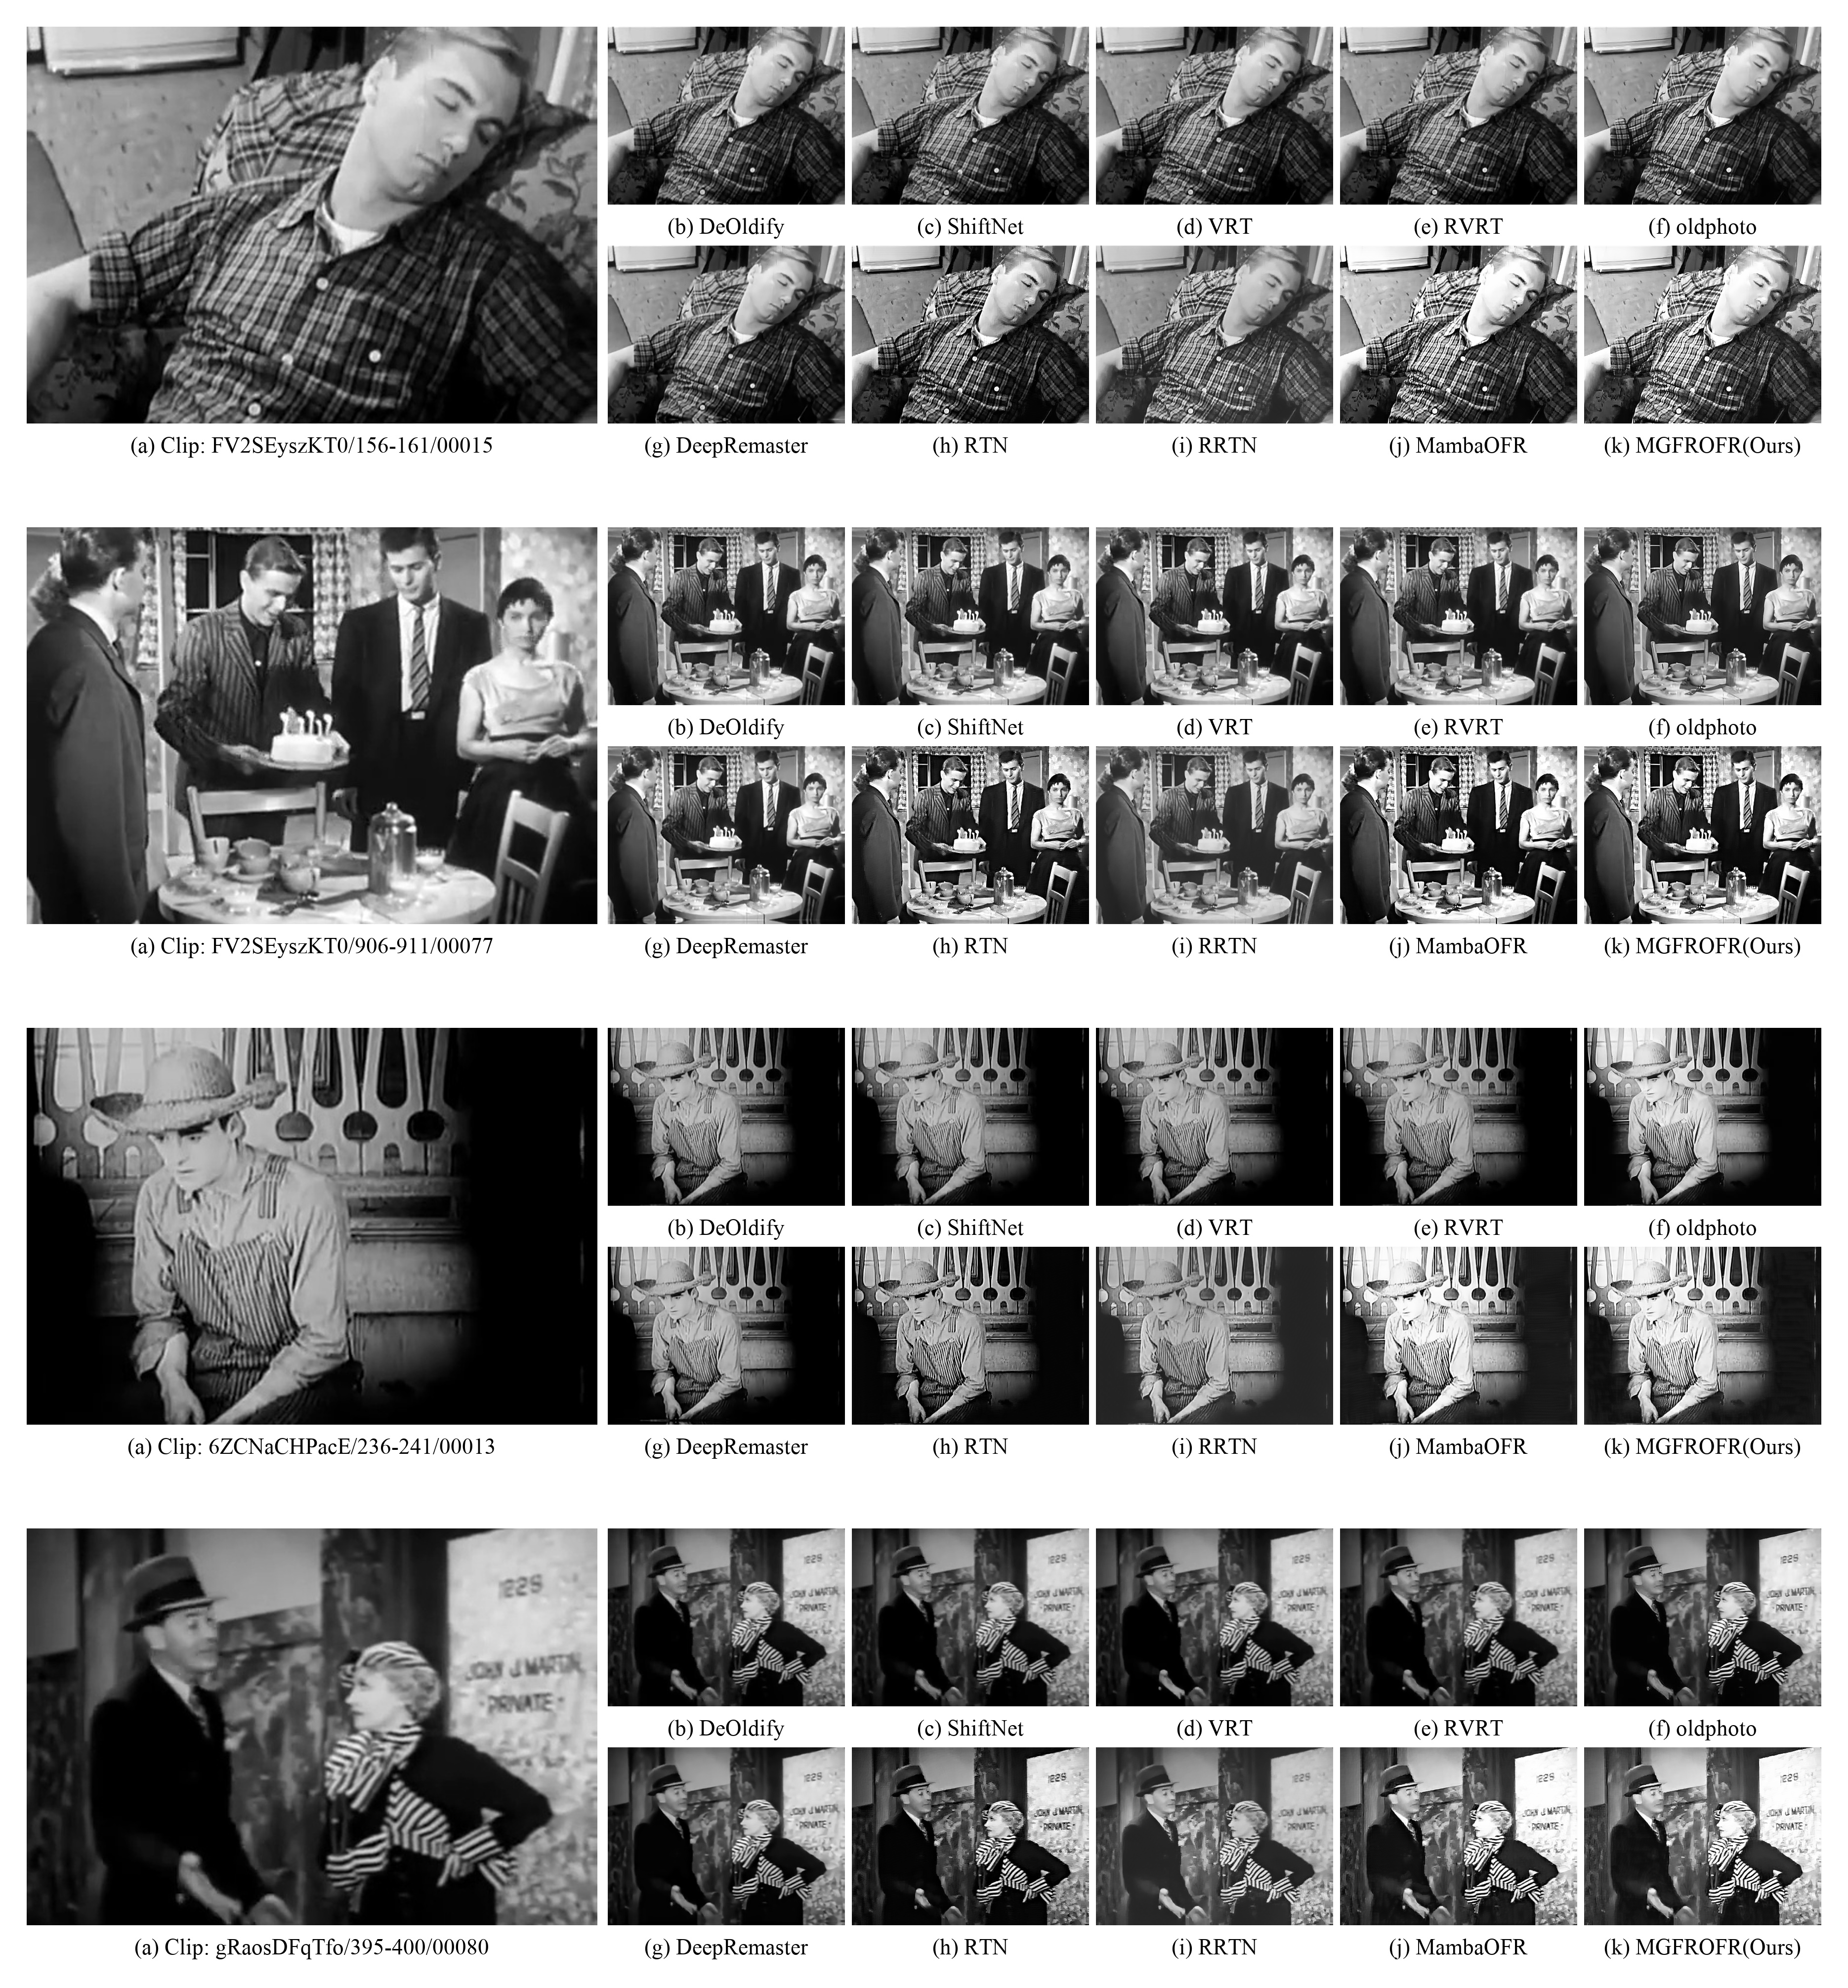
\includegraphics[width=0.95\textwidth]{figures/Fig5_SOTA_RealWorld_SRWOV_Qualitative.jpg}
\caption{Qualitative comparison on four representative SRWOV real-world clips. Each row shows one degraded input frame (a) and restoration results from DeOldify (b), ShiftNet (c), VRT (d), RVRT (e), OldPhoto (f), DeepRemaster (g), RTN (h), RRTN (i), MambaOFR (j), and MgfrOFR (Ours) (k). The selected clips cover facial close-ups, multi-person indoor scenes, strong vignetting, and high-contrast boundaries, illustrating that MgfrOFR suppresses residual old-film artifacts while preserving natural structure and local texture without relying on ground-truth references.\label{fig:qualitative_realworld}}
\end{figure}

Figure~\ref{fig:qualitative_realworld} compares visual results on four representative clips from the SRWOV real-world set: FV2SEyszKT0/\allowbreak 156--161/\allowbreak 00015, FV2SEyszKT0/\allowbreak 906--911/\allowbreak 00077, 6ZCNaCHPacE/\allowbreak 236--241/\allowbreak 00013, and gRaosDFqTfo/\allowbreak 395--400/\allowbreak 00080. Because no ground truth is available, the comparison focuses on visible artifact suppression, structural preservation, and naturalness. General video restoration methods reduce part of the photometric degradation but can leave residual scratches, stains, or contrast distortions. Image enhancement baselines may sharpen local texture while introducing over-enhancement around faces, clothing, and high-contrast boundaries. Compared with MambaOFR and the other OFR baselines, MgfrOFR more consistently preserves facial structure, fabric texture, object boundaries, and local contrast while suppressing residual old-film artifacts in these examples. These qualitative observations align with MgfrOFR's best NIQE and BRISQUE scores in Table~\ref{tab:realworld}; the CLIP-IQA+ ranking remains reported separately because it favors OldPhoto in the aggregate metric. MgfrOFR may still over-smooth very fine textures under extreme degradation, and severe motion blur can still cause flow-alignment errors; these cases are discussed in Section~\ref{subsec:failure}.



\FloatBarrier

\subsection{Ablation Study}
\label{subsec:ablation}

Table~\ref{tab:ablation} separates the effects of MGFE recalibration and RATR regularization. The setting names are kept consistent with Figure~\ref{fig:ablation_visual}. The +RATR only setting is a partial architectural control: MGFE branch descriptors are still computed as RATR ranking targets, while channel-wise recalibration is disabled.

\begin{table}[htbp]
\scriptsize
\caption{Ablation study on the SRWOV synthetic benchmark. The setting names match Figure~\ref{fig:ablation_visual}; ``MGFE''\ denotes channel-wise recalibration in this table. Best results are in \textbf{bold}.\label{tab:ablation}}
\centering
\begin{tabularx}{\textwidth}{>{\raggedright\arraybackslash}XccCCCC}
\toprule
\textbf{Setting} & \textbf{MGFE} & \textbf{RATR} & \textbf{PSNR$\uparrow$} & \textbf{SSIM$\uparrow$} & \textbf{LPIPS$\downarrow$} & \textbf{DISTS$\downarrow$} \\
\midrule
MambaOFR                        & Off & Off & 25.99 & 0.9059 & 0.0815 & 0.0822 \\
+MGFE only                 & On  & Off & 26.18 & 0.8960 & 0.1425 & 0.1132 \\
+RATR only                 & Off & On  & 26.84 & 0.9052 & 0.0963 & 0.0884 \\
MgfrOFR (Ours)             & On  & On  & \textbf{27.13} & \textbf{0.9237} & \textbf{0.0789} & \textbf{0.0653} \\
\bottomrule
\end{tabularx}
\end{table}

\noindent\textbf{Discussion.} MgfrOFR (Ours) improves MambaOFR by +1.14~dB in PSNR and achieves the best results across all four metrics. +MGFE only provides a small PSNR gain (+0.19~dB) but degrades LPIPS and DISTS, indicating that multi-granularity recalibration alone is insufficient. +RATR only gives a larger PSNR gain (+0.85~dB) and better perceptual balance. These results show that MGFE and RATR are complementary when used together.

\begin{figure}[htbp]
\centering
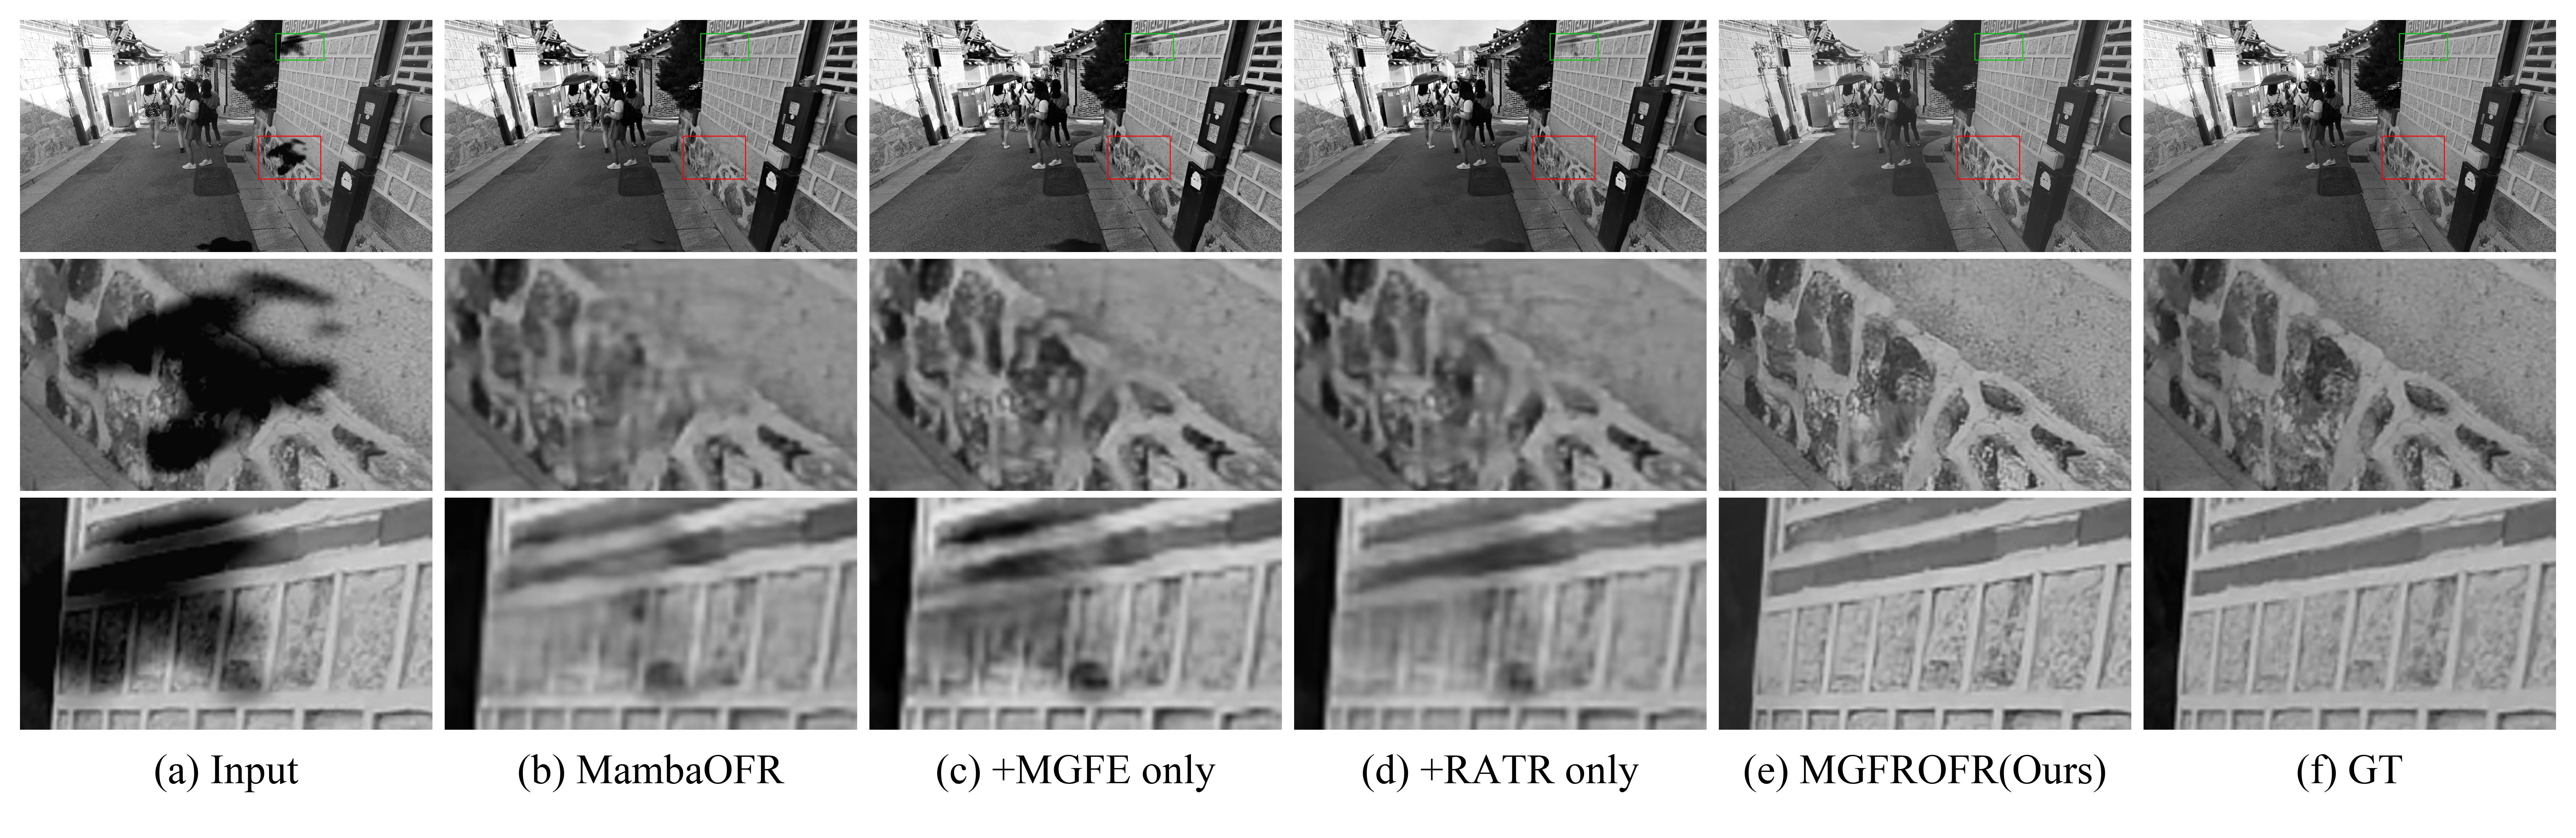
\includegraphics[width=0.95\textwidth]{figures/Fig6_Ablation_REDS_synthetic_Qualitative.jpg}
\caption{Visual ablation on REDS-based SRWOV synthetic data. \textbf{Top row:} full frames with red and green crop boxes marking the zoom regions. \textbf{Middle and bottom rows:} zoomed patches from the marked regions. From left to right, the restoration columns compare MambaOFR, +MGFE only, +RATR only, and MgfrOFR (Ours), with the degraded input and ground truth included as references. The comparison demonstrates that combining MGFE with RATR yields the cleanest local restoration among the ablated configurations in Table~\ref{tab:ablation}.\label{fig:ablation_visual}}
\end{figure}

\subsection{Hyperparameter Sensitivity}
\label{subsec:sensitivity}

We analyze MgfrOFR sensitivity to the main RATR and multi-granularity hyperparameters. Tables~\ref{tab:sensitivity_tau}--\ref{tab:sensitivity_granularity} report three groups: DKTau temperature $\tau$, RATR loss weights $\lambda_{\text{ratr}}$ and the intra/inter ratio, and the number of granularity branches $G$ and restoration tokens $M$. All experiments use the full MgfrOFR pipeline and are evaluated on the SRWOV synthetic benchmark.

\begin{figure}[H]
\centering
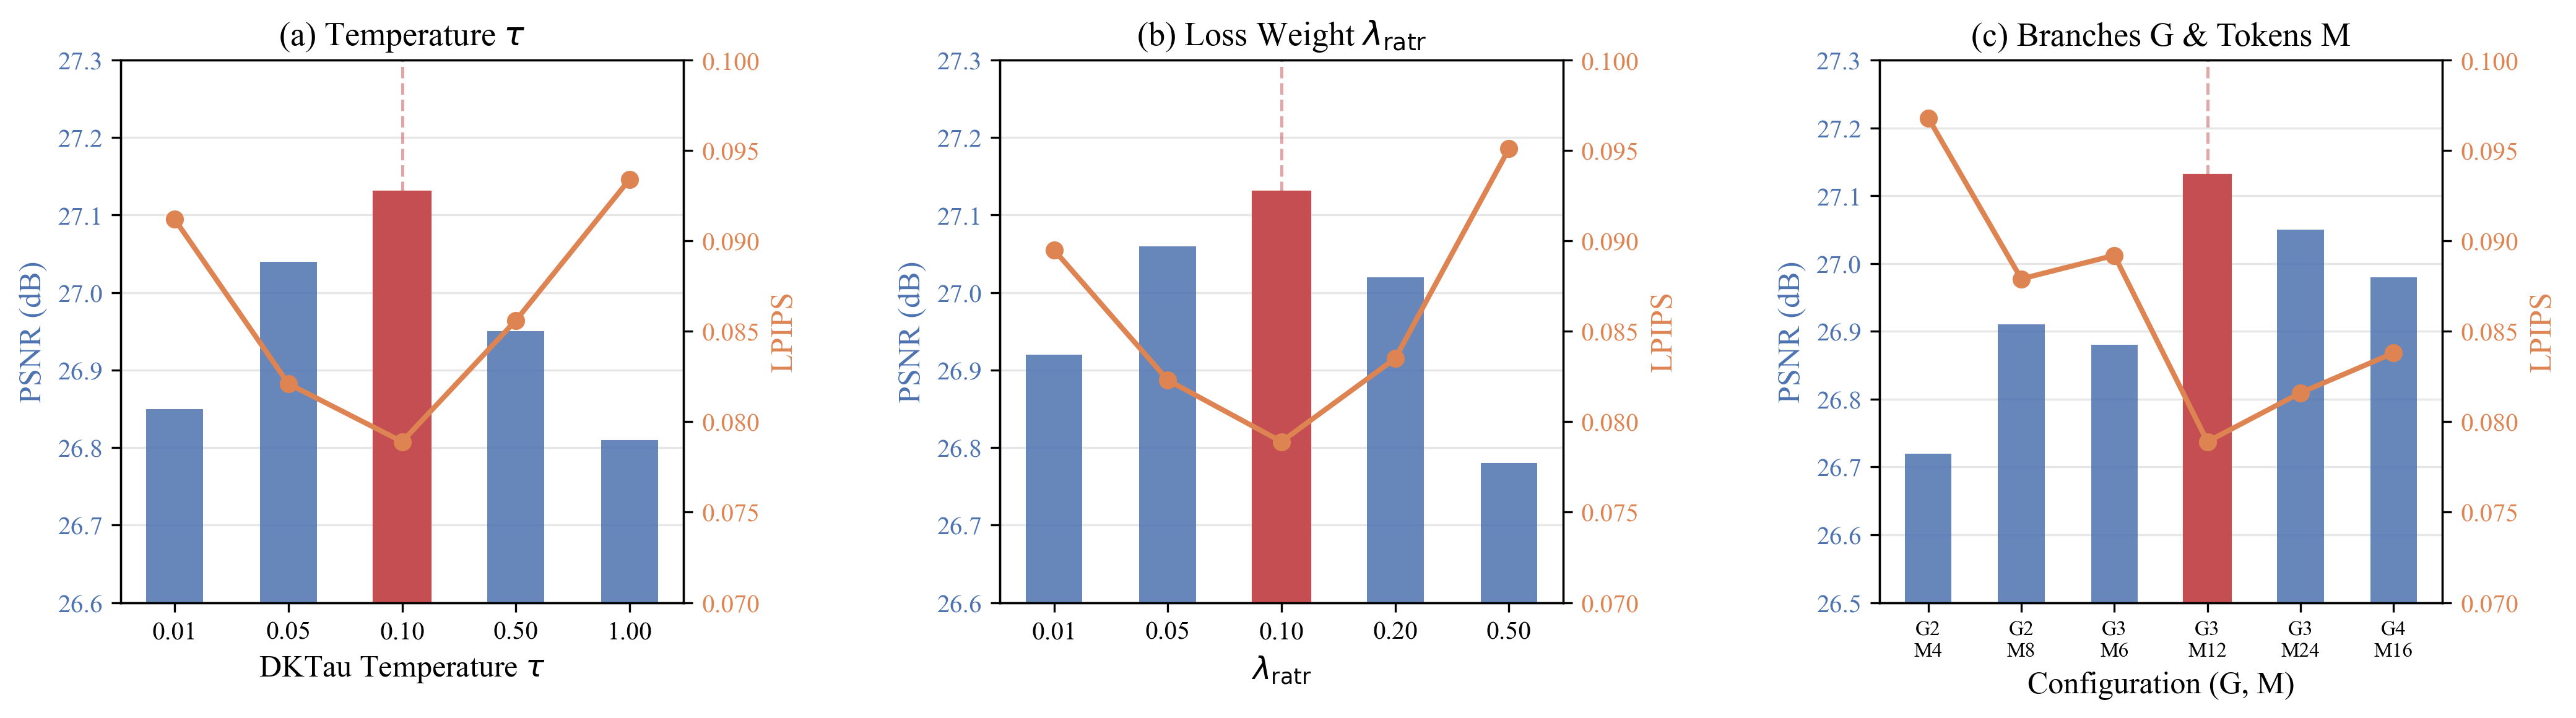
\includegraphics[width=0.95\textwidth]{figures/Fig7_sensitivity_analysis.png}
\caption{Hyperparameter sensitivity analysis. \textbf{Left:} DKTau temperature $\tau$. \textbf{Center:} RATR loss weight $\lambda_{\text{ratr}}$. \textbf{Right:} Number of branches $G$ and tokens $M$. The red bar (and the red dashed vertical line) marks the default configuration. PSNR is shown on the primary axis (bar); LPIPS on the secondary axis (line). The trends demonstrate that the default setting is a stable operating point rather than a brittle hyperparameter choice.\label{fig:sensitivity}}
\end{figure}

Figure~\ref{fig:sensitivity} summarizes the sensitivity trends across the three hyperparameter groups. Across the $\tau$ sweep, very small values make the ranking signal unstable, whereas overly large values oversmooth it. The RATR weight sweep follows the same pattern: weak regularization gives limited temporal constraint, while overly strong regularization reduces restoration flexibility. Together with the granularity sweep, these trends show that the default setting is a stable operating point within the tested range, without claiming global hyperparameter optimality.

\begin{table}[H]
\caption{Sensitivity to DKTau temperature $\tau$. The default setting is $\tau{=}0.1$.\label{tab:sensitivity_tau}}
\centering
\small
\begin{tabularx}{\textwidth}{CCCCC}
\toprule
$\tau$ & PSNR$\uparrow$ & SSIM$\uparrow$ & LPIPS$\downarrow$ & DISTS$\downarrow$ \\
\midrule
0.01  & 26.85 & 0.9068 & 0.0912 & 0.0871 \\
0.05  & 27.04 & 0.9121 & 0.0821 & 0.0825 \\
0.10  & \textbf{27.13} & \textbf{0.9237} & \textbf{0.0789} & \textbf{0.0653} \\
0.50  & 26.95 & 0.9098 & 0.0856 & 0.0843 \\
1.00  & 26.81 & 0.9054 & 0.0934 & 0.0878 \\
\bottomrule
\end{tabularx}
\end{table}

\begin{table}[H]
\caption{Sensitivity to RATR loss weights. Ratio denotes $\lambda_{\text{intra}}/\lambda_{\text{inter}}$; the default setting is $\lambda_{\text{ratr}}{=}0.1$ and ratio $2.0$.\label{tab:sensitivity_loss}}
\centering
\small
\begin{tabularx}{\textwidth}{ccCCCC}
\toprule
$\lambda_{\text{ratr}}$ & $\lambda_{\text{intra}}/\lambda_{\text{inter}}$ & PSNR$\uparrow$ & SSIM$\uparrow$ & LPIPS$\downarrow$ & DISTS$\downarrow$ \\
\midrule
0.01 & 2.0 & 26.92 & 0.9075 & 0.0895 & 0.0862 \\
0.05 & 2.0 & 27.06 & 0.9118 & 0.0823 & 0.0821 \\
0.10 & 2.0 & \textbf{27.13} & \textbf{0.9237} & \textbf{0.0789} & \textbf{0.0653} \\
0.20 & 2.0 & 27.02 & 0.9112 & 0.0835 & 0.0830 \\
0.50 & 2.0 & 26.78 & 0.9041 & 0.0951 & 0.0892 \\
\midrule
0.10 & 1.0 & 27.08 & 0.9125 & 0.0808 & 0.0815 \\
0.10 & 0.5 & 26.97 & 0.9095 & 0.0847 & 0.0839 \\
\bottomrule
\end{tabularx}
\end{table}

\begin{table}[H]
\caption{Sensitivity to the number of granularity branches $G$ and restoration tokens $M$. All configurations satisfy $M=k\cdot 2^{G-1}$; the default setting is $G{=}3$, $M{=}12$.\label{tab:sensitivity_granularity}}
\centering
\small
\begin{tabularx}{\textwidth}{ccCCCC}
\toprule
$G$ & $M$ & PSNR$\uparrow$ & SSIM$\uparrow$ & LPIPS$\downarrow$ & DISTS$\downarrow$ \\
\midrule
2 & 4   & 26.72 & 0.9032 & 0.0968 & 0.0895 \\
2 & 8   & 26.91 & 0.9082 & 0.0879 & 0.0856 \\
3 & 6   & 26.88 & 0.9070 & 0.0892 & 0.0864 \\
3 & 12  & \textbf{27.13} & \textbf{0.9237} & \textbf{0.0789} & \textbf{0.0653} \\
3 & 24  & 27.05 & 0.9115 & 0.0816 & 0.0822 \\
4 & 16  & 26.98 & 0.9101 & 0.0838 & 0.0835 \\
\bottomrule
\end{tabularx}
\end{table}

\FloatBarrier

\subsection{Complexity Analysis}
\label{subsec:complexity}

Table~\ref{tab:complexity} reports computational complexity under a unified measurement protocol in the same experimental environment described in Section~\ref{subsec:implementation}. Params/FLOPs for MambaOFR, MgfrOFR, and RTN are measured with PyTorch FlopCounterMode on a $1{\times}7{\times}3{\times}256{\times}256$ input, including the seven-frame forward pass and RAFT optical-flow front end. RRTN and DeepRemaster retain published Params/FLOPs because the released implementations are not directly compatible with this measurement path. Speed is reported as one mock training step divided by the seven frames in the clip.

\begin{table}[htbp]
\caption{Computational complexity comparison under the unified measurement protocol.\label{tab:complexity}}
\begin{tabularx}{\textwidth}{lCCCC}
\toprule
\textbf{Method} & \textbf{Params (M)} & \textbf{FLOPs (G)} & \textbf{Train Mem. (GB)$\downarrow$} & \textbf{Speed (ms/frame)$\downarrow$} \\
\midrule
DeepRemaster~\cite{iizuka2019deepremaster}  & 9.88  & 65.3   & 1.7   & 21.3  \\
RTN~\cite{wan2022rtn}                       & 6.18  & 2445.7 & 6.8   & 65.3  \\
RRTN~\cite{lin2024rrtn}                    & 7.54  & 3088.7 & 22.1  & 386.9 \\
MambaOFR~\cite{mao2025mambaofr}            & 3.49  & 2832.8 & 6.5   & 369.0 \\
\midrule
MgfrOFR (Ours)                              & 3.50  & 2846.9 & 7.0   & 396.9 \\
\bottomrule
\end{tabularx}
\end{table}

MgfrOFR adds 0.011M parameters (+0.32\%) and 14.1G FLOPs (+0.50\%) over MambaOFR. The added cost comes from restoration-token insertion, branch-specific token mixers in MGFE, and the training-only pairwise similarity computation in RATR. These additions keep MgfrOFR within the same computational order as MambaOFR while providing the restoration gains reported above.

\FloatBarrier
